\documentclass[12pt]{article}

% packages
\usepackage{kantlipsum}
\usepackage[margin=1in]{geometry}
\usepackage[labelfont=it]{caption}
\usepackage[table]{xcolor}
\usepackage{subcaption,framed,colortbl,multirow}
\usepackage{amsmath,amsthm,amssymb,wasysym,mathrsfs,mathtools}
\usepackage{tikz,graphicx,pgf,pgfplots}
\usetikzlibrary{arrows, angles, quotes, decorations.pathreplacing, math, patterns, calc}
\pgfplotsset{compat=1.16}

% custom commands
\newcommand{\N}{\mathbb{N}}
\newcommand{\Z}{\mathbb{Z}}
\newcommand{\I}{\mathbb{I}}
\newcommand{\R}{\mathbb{R}}
\newcommand{\Q}{\mathbb{Q}}
\newcommand{\C}{\mathbb{C}}
\newcommand{\F}{\mathbb{F}}
\newcommand{\p}{^{\prime}}
\newcommand{\powerset}{\raisebox{.15\baselineskip}{\Large\ensuremath{\wp}}}
\DeclarePairedDelimiter{\ceil}{\lceil}{\rceil}
\DeclarePairedDelimiter\floor{\lfloor}{\rfloor}

\setlength{\fboxsep}{4pt}
\newcommand{\exercise}[2]{\section*{Exercise #1}\begin{center}\framebox{\begin{minipage}{\textwidth-10pt}#2\end{minipage}}\end{center}}
\newcommand{\problem}[2]{\section*{Problem #1}\begin{center}\framebox{\begin{minipage}{\textwidth-10pt}#2\end{minipage}}\end{center}}
\newcommand{\generic}[2]{\section*{#1}\begin{center}\framebox{\begin{minipage}{\textwidth-10pt}#2\end{minipage}}\end{center}}

 
\begin{document}
 
\title{Assignment 4\\
    \large MATH CS 120FG Graph Theory I}
\author{Harry Coleman}
\date{February 18, 2020}
\maketitle


\generic{Question 1}{
    Let $x_{(r)} = x(x-1)\cdots (x-r+1).$ For a graph $G$, let $p_r(G)$ be the number of ways to partition $V(G)$ into $r$ independent sets, and let $n=|V(G)|$. Prove that $$\chi_G(x) = \sum_{r=1}^{n} p_r(G)x_{(r)}.$$
}

A proper $k$-coloring of a graph $G$ corresponds to a partition of $V(G)$ into $k$ independent sets. We consider groups of similarly colored vertices to correspond to parts of a partition. Given a particular partition of $V(G)$ into $r$ independent sets, we can find a proper $r$-coloring of $G$ by assigning different colors to each set of vertices in the partition. If we have $x$ colors to choose from, then there are $x$ possible color choices for the first set of vertices. The second set of vertices should be a different color from the first, so there are $x-1$ color choices. Each set of vertices has one less color to choose from than the previous. In total, for a given partition of $V(G)$ into $r$ independent sets and $x$ colors to choose from, there are
\[x_{(r)} = x(x-1)\cdots(x-(r-1))\]
possible colorings. So for a  given $x$ and $r$, with $p_r(G)$ ways to partition $V(G)$ into $r$ independent sets, there are
\[p_r(G)x_{(r)}\]
ways to color $G$ with exactly $r$ colors. In order to find $\chi_G(x)$, we want to consider all possible colorings of up to $x$ colors, so we look at all possible values of $r$ up to the number of vertices in $G$, that is,
\[\chi_G(X) = p_1(G)x_{(1)} + p_2(G)x_{(2)} + \cdots + p_n(G)x_{(n)},\]
\[\chi_G(x) = \sum_{r=1}^np_r(G)x_{(r)}.\]


\generic{Question 2}{
    Use Question 1 to prove that the chromatic polynomial $\chi_G(x)$ has no real root larger than $n-1$ where $n=|V(G)|.$
}

Since $\chi_G(x)$ is the number of ways to color the vertices of $G$ using at most $x$ colors, a real root of $\chi_G(x)$ would be a value of $x$ for which there are no proper $x$-colorings of $G$. For any graph with $n$ vertices, we can always find and $n$-coloring by making all vertices different colors. So for any value of $x$ which is greater than $n-1$, we will always have $\chi_G(x)$ be at least one, so no real value greater than $n-1$ could be a root of $\chi_G(x)$.


\generic{Question 3}{
    Use Question 1 to give a non-inductive proof that the coefficient of $x^{n-1}$ in $\chi_G(x)$ is $-m$ where $m=|E(G)|$ and $n=|V(G)|.$
}

In $\chi_G(x)$, we obtain $x^{n-1}$ terms in two ways. Firstly when $r=n-1$, we obtain from
\[p_{n-1}(G)x_{(n-1)} = p_{n-1}(G) \cdot x(x-1)\cdots(x-(n-2))\]
the term
\[p_{n-1}(G)x^{n-1}.\]
To find $p_{n-1}$, the number of ways to partition $V(G)$ into $n-1$ independent sets, we might consider starting with $n$ independent sets (each vertex on its own) and counting the number of ways to pair nonadjacent vertices. Since $G$ has $m$ edges, and there are $\binom{n}{2}$ possible edges between $n$ vertices, there are
\[\binom{n}{2} - m\]
pairs of nonadjacent vertices, and as many ways to partition $V(G)$ into $n-1$ independent sets. This gives us the value for $p_{n-1}(G)$. So we have
\[p_{n-1}(G)x^{n-1} = \left[ \binom{n}{2}-m\right]x^{n-1} = \left[ \frac{n(n-1)}{2}-m\right]x^{n-1}\]
as one of the $x^{n-1}$ terms. Secondly, when $r=n$, we obtain from
\[p_n(G)x_{(n)} = p_n(G) \cdot x(x-1)\cdots(x-(n-1))\]
multiple $x^{n-1}$ terms. Since there are $n$ factors of the form $(x+c)$, each $x^{n-1}$ term is produced by $x$'s from $n-1$ of the factors, and a constant $c$ from the remaining factor. This gives us an $x^{n-1}$ term with a coefficient $c$ for each $(x+c)$ factor. So from $r=n$, we obtain the terms
\[p_n(G)(-1x^{n-1} -2x^{n-1} -3x^{n-1} - \cdots - (n-1)x^{n-1}).\]
Which we can simplify to
\[[-p_n(G)(1+2+3+\cdots +(n-1))]x^{n-1},\]
\[\left[-p_n(G)\frac{n(n-1)}{2}\right]x^{n-1}.\]
Since $p_n$ is the number of ways to partition $V(G)$ into $n$ independent sets, and $n=|V(G)|$, then $p_n=1$. This makes sense because the only way to partition $V(G)$ into $n$ independent sets is to make each set contain exactly one vertex. So we have
\[\left[-\frac{n(n-1)}{2}\right]x^{n-1}\]
from $r=n$ and
\[\left[ \frac{n(n-1)}{2}-m\right]x^{n-1}\]
from $r=n-1$, which we combine to find the $x^{n-1}$ term of $\chi_G(X)$,
\[\left[ \frac{n(n-1)}{2}-m\right]x^{n-1} + \left[-\frac{n(n-1)}{2}\right]x^{n-1},\]
\[-mx^{n-1}.\]
So $-m$ is the coefficient of the $x^{n-1}$ term.



\generic{Question 4}{
    For $n\geq 1$, let $G_n$ be the ladder graph on $2n$ vertices with $3n-2$ edges ($G_4$ is pictured below). Prove that $$\chi_{G_n}(x) = (x^2-3x+3)^{n-1}x(x-1).$$ 
    \begin{center}
    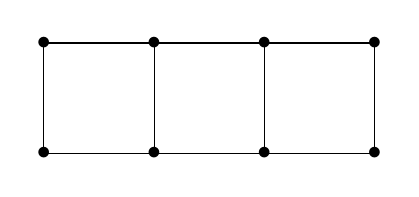
\begin{tikzpicture} [scale=0.7]
         \draw (0,0) node {$\bullet$};
         \draw (2,0) node {$\bullet$};
        \draw (4,0) node {$\bullet$}; 	
        \draw (6,0) node {$\bullet$}; 
        
         \draw (0,2) node {$\bullet$};
         \draw (2,2) node {$\bullet$};
        \draw (4,2) node {$\bullet$}; 	
        \draw (6,2) node {$\bullet$}; 
        
        \draw (0,0) -- (6,0);
        \draw (0,2) -- (6,2);
        \draw (0,0) -- (0,2);
        \draw (2,0) -- (2,2);
        \draw (4,0) -- (4,2);
        \draw (6,0) -- (6,2);
    \end{tikzpicture}
    \end{center}
}

We will show inductively that
\[\chi_{G_n}(x) = (x^2 - 3x + 3)^{n-1}x(x-1).\]
The base case of $n=1$ is easily shown with the formula from Question 1 applied to the graph $G_1$ (which is two vertices with one edge between them). So $p_1(G_1)=0$ since the two vertices are not independent, and $p_2(G_1)=1$ since there is only one way to split up the two vertices into two sets. So we solve to find
\[\chi_{G_1}(x) = \sum_{r=1}^2p_r(G_1)x_{(r)},\]
\[\chi_{G_1}(x) = p_1(G_1)x_{(1)} + p_2(G_1)x_{(2)},\]
\[\chi_{G_1}(x) = 0x + 1x(x-1),\]
\[\chi_{G_1}(x) = (x^2-3x+3)^0x(x-1).\]

For the inductive step, we will assume that the formula is true for some $n$, and then show that it is also true for $n+1$. Consider the graph of $G_{n+1}$ and how it contains the graph $G_n$.

\begin{center}
    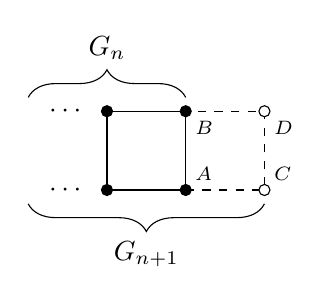
\begin{tikzpicture}
        \foreach \x/\y in {0/0, 0/1, 1/0, 1/1} {
            \draw[fill=black] (\x,\y) circle (2pt);
        }
        \draw[] (0,0) -- (0,1) -- (1,1) -- (1,0) -- (0,0);
        \draw[dashed] (1,0) -- (2,0) -- (2,1) -- (1,1);
        \draw[fill=white] (2,0) circle (2pt);
        \draw[fill=white] (2,1) circle (2pt);
        
        \draw[] (-0.5,0) node[]{$\cdots$};
        \draw[] (-0.5,1) node[]{$\cdots$};
        
        \draw[decorate,decoration={brace,amplitude=10pt}, yshift=5pt] (-1, 1) -- (1,1) node[midway, anchor=south, yshift=10pt]{$G_n$};
        \draw[decorate,decoration={brace,amplitude=10pt,mirror}, yshift=-5pt] (-1, 0) -- (2,0) node[midway, anchor=north, yshift=-10pt]{$G_{n+1}$};
        
        \draw[] (1,0) node[anchor=south west]{\scriptsize $A$};
        \draw[] (1,1) node[anchor=north west]{\scriptsize $B$};
        \draw[] (2,0) node[anchor=south west]{\scriptsize $C$};
        \draw[] (2,1) node[anchor=north west]{\scriptsize $D$};

    \end{tikzpicture}
\end{center}

To find $\chi_{G_{n+1}}(x)$, we will use the $x$-colorings of $G_n$. Given a particular $x$-coloring of $G_n$, we can obtain a number of $x$-colorings on $G_{n+1}$ by picking colors for vertices $C$ and $D$. For vertex $C$, we can pick any color except for that of $A$, which gives us $x-1$ options; $x-2$ of which are different from $B$ and 1 of which is the same as $B$. For vertex $D$, if $C$ is different from $B$, then there are $x-2$ options, and if $C$ and $B$ are the same, there are $x-1$ options. this gives us
\[(x-2)(x-2) + (x-1) = x^2 - 3x + 3\]
possible ways to make an $x$-coloring of $G_{n+1}$ from an $x$-coloring of $G_n$. So
\[\chi_{G_{n+1}}(x) = \chi_{G_n}(x) \cdot (x^2 - 3x + 3),\]
and from the inductive hypothesis,
\[\chi_{G_{n+1}}(x) = (x^2 - 3x + 3)^{n-1}x(x-1) \cdot (x^2 - 3x + 3),\]
\[\chi_{G_{n+1}}(x) = (x^2 - 3x + 3)^nx(x-1).\]
Which completes the inductive step. So the formula is true for all $n$.


\generic{Question 5}{
    Prove that any tree has at most one perfect matching.
}

We will show that any tree has at most one perfect matching by induction on the number of vertices $n$. We provide two base cases, since our inductive step will increment $n$ by 2. The case of $n=1$ is clearly true since a tree on one vertex has no edges and therefore no matchings. The case of $n=2$ is also true, since a tree on two vertices has one edge, and thus one matching.

For the inductive step, we will assume that for any tree on $n$ vertices, there is at most one perfect matching. Let $T$ be a tree on $n+2$ vertices. Let vertex $v$ be a leaf in $T$ which is connected to vertex $u$ by edge $e$. Since $v$ is a leaf, it has only one incident edge, $e$. This means that any perfect matching on $T$ must include $e$, and therefore also includes a perfect matching on $T-\{u,v\}$, which is $T$ without the vertices $u$ and $v$. So $T$ has at most as many perfect matchings as $T-\{u,v\}$, which is a tree on $n$ vertices. So by the inductive hypothesis, $T-\{u,v\}$ has at most one perfect matching, and so does $T$.

Since the base case covered $n=1$ and $n=2$, and the inductive step incremented by $2$, for any natural number $n$, a tree on $n$ vertices has at most one perfect matching. So any tree has at most one perfect matching.



\generic{Question 6}{
    A \emph{permutation} matrix is an $n\times n$ matrix with entries from $\{0,1\}$ and where each row and each column has exactly one $1$. 

    Prove that if $A$ is an $n\times n$ matrix with entries from $\{0,1\}$ such that each row and each column has exactly $k$ $1$'s, then $A$ is the sum of $k$ permutation matrices.   
}

For any $n\times n$ matrix $M$ with entries from $\{0,1\}$, we will define the related bipartite graph $G_M$ between the set of rows $R=\{r_1,\dots,r_n\}$ and the set of columns $C=\{c_1,\dots,c_n\}$. If $M_{ij} = 1$, then $r_i$ and $c_j$ are adjacent in $G_M$, and not adjacent otherwise. For example, given the matrix
\[M = \begin{bmatrix}
    1 & 1 & 0 & 0 \\
    0 & 0 & 1 & 1 \\
    1 & 0 & 1 & 0 \\
    0 & 1 & 0 & 1 \\
\end{bmatrix},\]
we define the bipartite graph $G_M$:
\begin{center}
    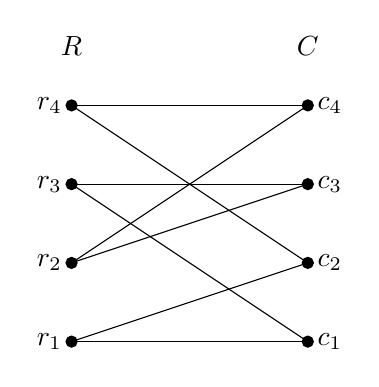
\begin{tikzpicture}
        \foreach \y in {1, 2, 3, 4} {
            \draw[fill=black] (0,\y) circle (2pt) node[anchor=east]{$r_\y$};
            \draw[fill=black] (3,\y) circle (2pt) node[anchor=west]{$c_\y$};
        }
        \draw[] (0,1) -- (3,1);
        \draw[] (0,1) -- (3,2);
        \draw[] (0,2) -- (3,3);
        \draw[] (0,2) -- (3,4);
        \draw[] (0,3) -- (3,1);
        \draw[] (0,3) -- (3,3);
        \draw[] (0,4) -- (3,2);
        \draw[] (0,4) -- (3,4);
        
        \draw[] (0,4.75) node[]{$R$};
        \draw[] (3,4.75) node[]{$C$};
    \end{tikzpicture}
\end{center}

Adding two matrices (which, along with their sum, have entries from $\{0,1\}$) would correspond to combining the edges present in each of the graphs.

The graph of a permutation matrix would have a related graph which would be a perfect matching of $R$ into $C$, since each row and column has exactly one 1.

A matrix which could be expressed as the sum of a permutation matrix and another matrix would have a perfect matching of rows into columns; that perfect matching representing the permutation matrix.

We will show by induction on $k$ that any $n\times n$ matrix $A$ with entries from $\{0,1\}$ such that each row and each column has exactly $k$ 1's, then $A$ is the sum of $k$ permutation matrices. For the base case $k=1$, $A$ is is a permutation matrix, and so is the sum of permutation matrices.

For the inductive step, we'll assume that for some $k$, the property holds. Let $A$ be an $n\times n$ matrix with entries from $\{0,1\}$ such that each row and column has exactly $k+1$ 1's, and $G_A$ be the related bipartite graph of vertex sets $R$ and $C$. We want to show that there is a perfect matching of $R$ into $C$, which would tell us that $A$ is the sum of a permutation matrix and a matrix in which each row and column has exactly $k$ 1's. 

For there to be a perfect matching, the condition for Hall's theorem must be met. That is, for any subset $S \subseteq R$, $|S| \leq |N(S)|$. Let $S\subseteq R$. Since each $r_i$ is connected to exactly $k$ vertices in $C$, there are $|S|k$ edges coming from $S$. So the average degree of vertices in $N(S)$ with respect to vertices in $S$ is
\[\frac{|S|k}{|N(S)|}.\]
which must be less than $k$, so
\[\frac{|S|k}{|N(S)|} \leq k,\]
\[|S| \leq |N(S)|.\]
So Hall's theorem holds, and a perfect matching exists. Which completes the inductive proof.



\end{document}